\chapter{Polar Map Construction}

To enable population-level statistical analysis of post-infarction scar geometry, individual
three-dimensional scar surfaces must be projected onto a common two-dimensional
representation that preserves anatomical meaning across patients. This chapter describes
the pipeline that constructs this projection.

\section{Rationale: Why Flatten to 2D}

A statistical shape model of scar requires point-to-point correspondence across patients:
every patient's scar must be represented in a common coordinate frame so that
corresponding locations can be compared. An initial approach would be to establish this
correspondence directly on the three-dimensional LV surface, for instance by registering all
LV meshes to a common template and mapping scar labels through the deformation field.
However, exploratory analysis of the cohort revealed that post-infarction scar is extremely
variable in position, extent, and shape. Scar can appear in any coronary territory, at any
longitudinal level, and with transmural extent ranging from thin subendocardial ribbons to
full-thickness replacement.

A natural idea would have been to build the statistical shape model directly on the scar
tissue, treating each patient's scar as a surface. However, this proved impractical because
scar tissue presents highly heterogeneous three-dimensional morphologies across patients:
some infarctions produce concave apical geometries, others present flat surfaces, and yet
others exhibit convex or irregular shapes. This morphological diversity means that no single
reference scar shape exists onto which all patients could be mapped.

The bull's-eye or circumferential polar map provides a solution. By projecting the
three-dimensional LV surface onto a two-dimensional disk using cylindrical coordinates
anchored to the long axis and the septal reference, every patient's scar is expressed in the
same $(s, \theta)$ frame regardless of ventricular size, shape, or orientation. This
representation naturally provides inter-patient correspondence and reduces the problem to a
two-dimensional image amenable to standard statistical analysis.

\section{Apex Detection via Multi-Candidate Convex-Hull Search}

The apex is the geometric anchor of the entire polar map pipeline. Rather than relying on a
single principal component direction, the algorithm evaluates multiple candidate search
directions and selects the one that most clearly identifies the pointed apical tip of the left
ventricle.

The algorithm extracts the vertex coordinates of the full LV shell mesh and computes their
centroid. The centred point cloud is factored by singular value decomposition (SVD), yielding
principal components ordered by decreasing singular value. A separate SVD is performed
on the RV point cloud and its first principal component is also extracted. These three
directions---LV PC1, LV PC2, and RV PC1---form the list of candidate search directions.

For each candidate direction $\mathbf{a}$, let $\mathbf{c}$ denote the LV centroid and
$P_\text{hull}$ the set of convex-hull vertices. Each hull vertex $\mathbf{p}_i$ is projected
onto the candidate direction relative to the centroid, yielding a signed scalar distance
$d_i = (\mathbf{p}_i - \mathbf{c}) \cdot \mathbf{a}$. The apex candidate is the hull vertex
with the largest absolute projection. To score how pointed this candidate is, a half-span $H$
is computed from the full vertex set: $H = (d_\text{max} - d_\text{min}) / 2$. The
eccentricity is then $e = |d_\text{apex}| / H$. The candidate direction yielding the highest
eccentricity is selected.

LV PC1 captures the apex-to-base elongation in the majority of cases. However, pathological
ventricular remodelling or mesh truncation can make the LV point cloud nearly isotropic,
causing PC1 to align with circumferential rather than longitudinal variance. RV PC1 is
included because the RV's strongly elongated crescent shape reliably recovers the
base-to-apex direction even when the LV shape is unfavourable. LV PC2 provides an
additional fallback for the rarer cases where the true long axis is captured by the second
rather than the first principal direction.

\section{Long-Axis and Septal Reference}

Once the apex has been detected, the long axis is constructed as the unit vector pointing
from the detected apex toward the LV centroid. This construction guarantees that the axis
passes through the apex by definition, that the direction is unambiguously from apex toward
base, and that the result is entirely LV-intrinsic regardless of which search direction found the
apex.

A circumferential zero-angle must be established so that the anterior, septal, inferior, and
lateral walls map to consistent angular positions across patients. The septal direction is
computed from the spatial relationship between the LV and RV centroids, both restricted to a
basal band spanning 50 to 90 percent of the apex-to-base distance to avoid bias from the
apically-extending RV free wall. The raw direction vector from the LV centroid to the RV
centroid is projected onto the plane perpendicular to the long axis and normalised to a unit
vector.

\section{Polar Coordinate Computation}

Every point on the LV surface is mapped to two cylindrical polar coordinates. The
longitudinal coordinate $s$ is obtained by projecting the displacement from the apex onto the
long axis and normalising by the total span, so that $s = 0$ at the apex and $s = 1$ at the base:
\begin{equation}
    s = \frac{(\mathbf{p} - \mathbf{apex}) \cdot \mathbf{axis}}{\text{span}}.
    \label{eq:longcoord}
\end{equation}
The circumferential angle $\theta$ is measured relative to the septal reference direction. The
continuous coordinates are discretised into a $64 \times 128$ (radial $\times$ angular) grid,
giving approximately 6 vertices per bin for a typical LV shell mesh of ${\sim}50{,}000$ vertices.

The bull's-eye grid is partitioned into the AHA 17-segment model \cite{cerqueira2002} using four concentric rings:
the apical cap ($s \in [0, 0.25]$, segment 17), the apical ring ($s \in [0.25, 0.50]$, four
$90^{\circ}$ sectors), the mid-cavity ring ($s \in [0.50, 0.75]$, six $60^{\circ}$ sectors), and
the basal ring ($s \in [0.75, 1.00]$, six $60^{\circ}$ sectors).

\begin{figure}[htbp]
    \centering
    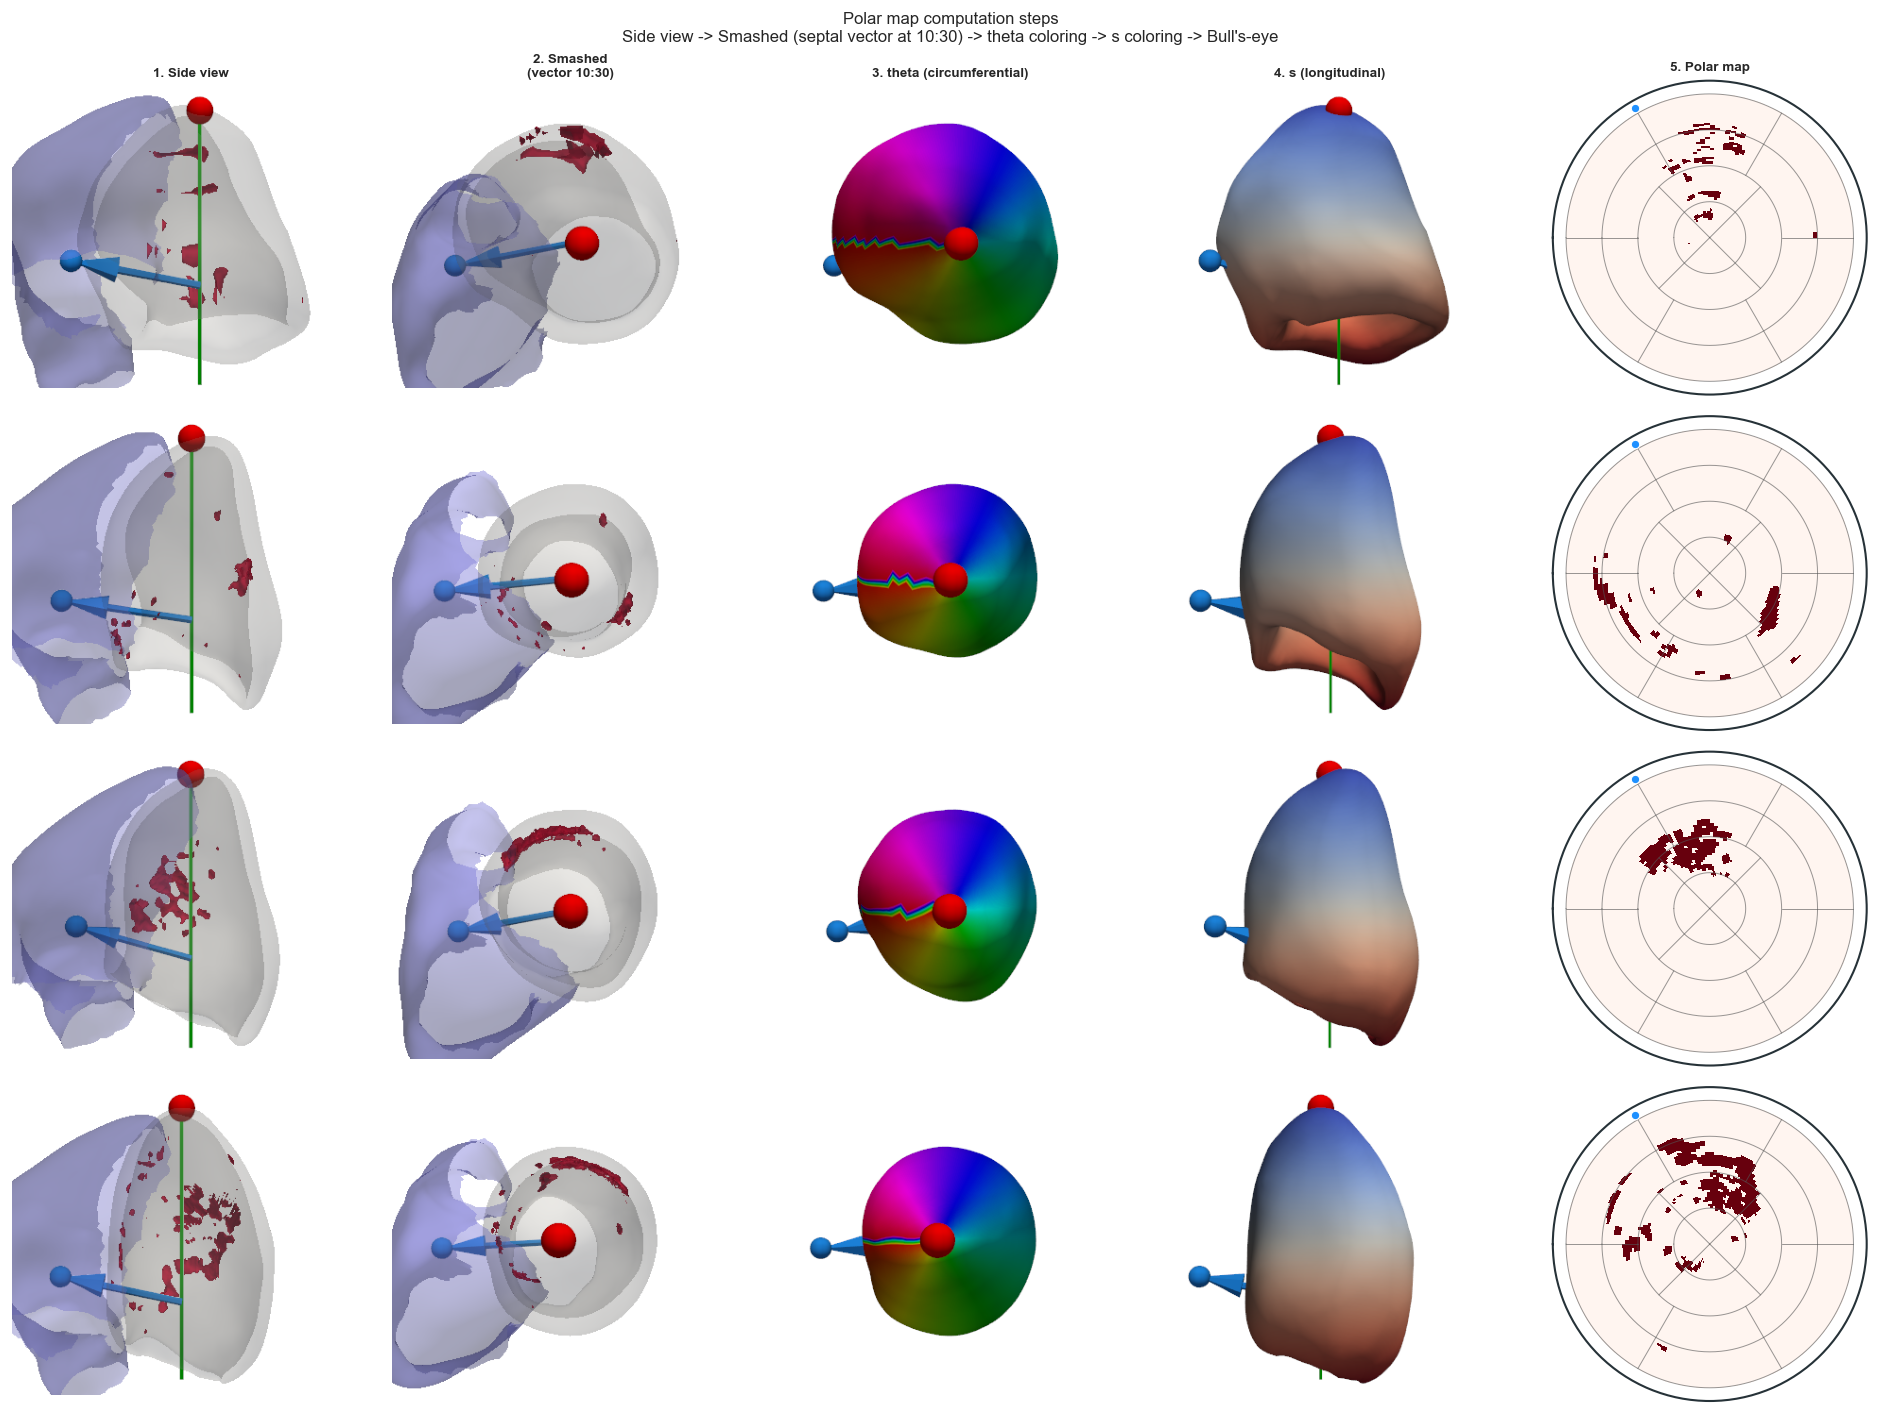
\includegraphics[width=\textwidth]{figures/polar_map_steps}
    \caption{Polar map projection pipeline. From left to right: original 3D LV and RV meshes; long-axis detection and apex-down re-orientation; longitudinal coordinate $s$ computed apex-to-base; circumferential angle $\theta$ anchored to the septal reference; final 2D bull's-eye polar map with AHA 17-segment overlay.}
    \label{fig:polarmaps2}
\end{figure}

\section{Scar Projection Methods}

Three complementary methods are used to project scar onto the polar grid. The
\textbf{vertex-based method} assigns a binary label to each polar bin: a bin is marked as
scarred if at least one core-zone vertex projects into it. When averaged across patients, each
grid value represents the fraction of patients with scar in that location. This method is the
primary representation because it is reversible (supports round-trip 3D$\to$2D$\to$3D
mapping), separates location from intensity, and transfers cleanly to target meshes with
different vertex densities.

The \textbf{area-based method} accumulates triangle surface areas per bin (mm$^2$),
capturing absolute scar burden. The \textbf{coverage method} divides CZ area by total LV
area per bin, removing bin-size and LV-size bias. Consistency between all three approaches
was verified to ensure that findings are not artefacts of the binary representation.

\section{Polar Map Verification}

To provide an independent qualitative assessment of anatomical plausibility, the polar maps
produced by the proposed pipeline were compared against those generated by the
conformal flattening method of N\'{u}\~{n}ez Garc\'{i}a \cite{nunez2018} for four representative cases. Both methods
operated on the same Endo Layer mesh, which is required as input by the reference
flattening script; the main pipeline uses the full LV shell for axis and span estimation in all
other analyses, and this difference introduces a small systematic variation in longitudinal
span that is independent of the comparison's primary findings.

One methodological difference concerns scar detection: the proposed method projects Core
Surface vertices directly onto the polar grid, whereas the reference method proximity-labels
endocardial surface points within a tolerance derived from the Core Surface mesh spacing,
then maps those labelled points using the 2D flat coordinates. A further distinction concerns
the radial mapping: the reference method applies a radial displacement transform of the form
$r_\text{new} = r^{1/3}$ to the conformally flattened disk \cite{paun2017}, which
redistributes points outward and produces denser coverage near the basal ring. The
proposed pipeline uses a linear longitudinal mapping and therefore does not exhibit this
redistribution. Prior to visual comparison, both polar maps were aligned to the same septal
reference direction.
